\chapter{Methodology}
    \label{chap:methodology}
    
In this chapter, we will be discussing the research methodology of the project, then explain the implementation of the proposed model and the metrics which will be used in experiments.
    
\section{Research methodology}

The EOT framework presented in subsection \ref{subsec:eot} is highly effective at creating robust adversarial noise for 3D-rendered objects. This is despite the fact it is training on renders of the object with a random position and angle. In EOT, the transformation from the texture to the rendered image is represented as a simple linear transformation. At the same time, generative models have proven to be capable at learning a distribution for generating large 256x256 images \cite{big_gan}, especially benefiting from having significantly more parameters. Therefore, our intuition is that with the proper training hyper-parameters and architecture, a generative model should be able to learn to create adversarial textures. Since the transformation representing 3D rendering is linear, it should be an insurmountable obstacle for training the generator.

Moreover, the black-box generative model in subsection \ref{subsubsec:zheng} can be easily combined with the EOT framework for making adversarial objects in subsection \ref{subsec:eot}, by placing a differentiable rendering pipeline between the generator and the simulator.

The research hypothesis of this project is the following: 

\textit{It is possible to use a generative neural network to create 3D-rendered adversarial objects in the targeted black-box setting that have a targeted fooling rate of at least 50\% on a victim CNN classifier for object recognition.}

\bigbreak
The targeted fooling rate metric is explained later in section \ref{sec:analytic_techniques}.

This is a quantitative experimental research project. The model proposed in section \ref{sec:architecture_design} creates 3D-rendered objects, and pictures of those objects will be given to various neural network classifiers. The predicted label will be compared against the correct label and the adversarial target label to evaluate the effectiveness of the proposed method. We will mainly be using a circulatory research process, to try Further details on the experiments are found in subsection \ref{sec:experiment_design}.

\section{Implementation of EOT}

\section{Implementation of Zheng et al.'s model}

\section{Architecture design of G-EOT}
    \label{sec:architecture_design}
    
The proposed G-EOT model is almost the same generative model presented in subsection \ref{subsubsec:zheng}, except that it has elements of the EOT framework \cite{athalye} added to it. The key difference is that the generator produces adversarial perturbations for a 2D texture rather than an image of an object, as you can see in figure \ref{fig:proposed_model}. The adversarial texture is then rendered as a 3D object, and an image of the rendered object is then given to the simulator and victim model.

\begin{figure}[h]
    \centering
    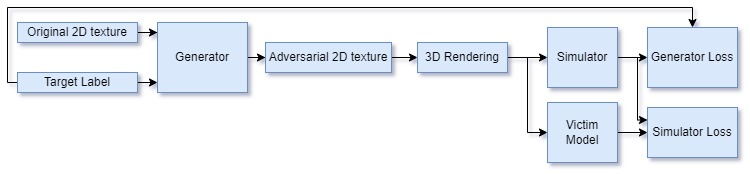
\includegraphics[width=1\textwidth]{graphics/model.jpg}
    \caption{The architecture of the proposed generative model.}
    \label{fig:proposed_model}
\end{figure}

The 3D rendering simulates a variety of transformations such as 3D rotation, translation, varying camera distance, different background and lighting conditions, and 3D printer errors, just like it was done in the EOT framework from subsection \ref{subsec:eot}. I am using the same distribution $T$ of transformation functions as \cite{athalye} did. The mini-batches used at each training step shall be constructed as described in the penultimate paragraph of subsection \ref{subsec:eot}.

The generator will have the same structure as the one in figure \ref{fig:zheng_generator} in subsection \ref{subsubsec:zheng}. The simulator will again be a CNN, and I will experiment with the 4 simulator architectures used in \cite{zheng_black_box_GAN}. Moreover, the simulator will be trained in the same way as subsection \ref{subsubsec:zheng} describes. The generator will also be trained as equation \ref{eq:generator_loss} on page \pageref{eq:generator_loss} describes, except that the penalty term will be replaced by:

\begin{equation}
    \begin{aligned}
    \beta\|LAB(t(x + G(x,z))) - LAB(t(x))\|_2
    \end{aligned}
\end{equation}

\noindent because the $LAB$ space distance metric encourages imperceptibility to the human eye.

I chose to use EOT \cite{athalye} rather than $\textrm{RP}_2$ \cite{evtimov_road_signs} because it is a lot more convenient, for reasons named in subsection \ref{subsubsec:rp2_results}. Furthermore, the synthetic transformation functions for 3D rendered objects can accurately simulate real-world transformations \cite{athalye}.

Regarding the 3D renderer, it is to take a 2D texture and render it as a 3D object. It supports 3D rotation, translation, perspective projection, different background colours, and additive and multiplicative lighting. Moreover, since the transformation functions $t(\cdot)$ simulate 3D rendering and must be differentiable, the chosen renderer must return the texture-space coordinates. Athalye \textit{et al.} \cite{athalye} do not say which specific renderer they used, they just modified an existing renderer to return that information. This project will use ModernGL \footnote{https://github.com/moderngl/moderngl}, a Python wrapper around OpenGL which allows the user to render .obj files with textures.

\section{Analytic techniques}
    \label{sec:analytic_techniques}
    
For Dr Deng: The CSCM-10 lecture on the dissertation said we should have a section on analytic techniques in the methodology chapter. Is the below what they meant by "analytic techniques"?
    
Unless otherwise specified, each experiment will use both of the following metrics to evaluate the proposed attack's success:

\begin{itemize}
    \item \textbf{Targeted Fool Rate (TFR):} the percentage of adversarial examples that are classified by the victim model as the desired target label.
    \item \textbf{Untargeted Fool Rate (UFR):} the percentage of adversarial examples that are classified by the victim model as any incorrect label. It is relevant because if the attack induces a misclassification, even if it is not the desired target label, then it is still potentially dangerous.
\end{itemize}
